\documentclass[a4paper,12pt]{article}
\usepackage[utf8]{inputenc}
\usepackage[french]{babel}
\usepackage[T1]{fontenc}
\usepackage[top=2cm,bottom=2cm,left=2cm,right=2cm]{geometry}
\usepackage{graphicx}
\usepackage{wrapfig}
\usepackage{url}

\begin{document}

\begin{titlepage}
	\begin{center}
		\Large{Année universitaire 2016-2017}\\
		\Large{Université de Caen Basse-Normandie}\\[1cm]
		
		\huge{Rapport sur la progression du projet de création d'une IDE}\\
		\vspace{3cm}
		
		Alexis Carreau\\
		Thomas Lécluse\\
		Emma Mauger\\
		Théo Sarrazin\\
		
	\normalsize{\textit{ ~ L2 Informatique}}\\
		\medskip
		\vspace{2cm}
		
	\end{center}
\end{titlepage}

\tableofcontents
\newpage

\section{Séance 1, 09/09/16}

	\subsection{Un IDE, qu'est-ce que c'est ?}

		\subsubsection{Définition}

			Un  IDE   ou  Environnement   de  Développement   Intégré  (Integrated
			Development Environment) est un logiciel  qui fournit des facilités au
			programmeur pour le développement logiciel. Il a pour but de maximiser
			la productivité du programmeur.

		\subsubsection{Que contient-il ?}

			Un IDE contient généralement un  éditeur de texte, un interpréteur, un
			debugger et un compilateur.

		\subsubsection*{L'éditeur de texte}

			L'éditeur de texte présente une zone  de saisie de texte. Il ne permet
			pas la mise en forme de ce dernier.

		\subsubsection*{L'interpréteur}

			L'interpréteur analyse,  traduit et  exécute les  instructions écrites
			dans  un   langage  informatique.  Ces  opérations   d'analyse  et  de
			traduction sont effectuées à chaque fois que l'on décide d'exécuter le
			programme.

		\subsubsection*{Le debugger}

			Un  debugger est  un  logiciel  qui permet  d'analyser  les bugs  d'un
			programme (tels que  des erreurs de syntaxe). Il  permet d'exécuter le
			programme pas-à-pas,  d'arrêter le programme,  de l'observer et  de le
			contrôler.

		\subsubsection*{Le compilateur}

			Un compilateur est un programme informatique qui transforme un code source écrit dans un langage de programmation 					(langage source) en un autre langage (langage cible), afin qu'il puisse être interprété par la machine (qui ne 						comprend un langage dit de bas niveau et traductible en binaire).

			Les langages utilisés pour programmer sont dits "de haut niveau" (car facilement compréhensible par l'homme), tandis 				que les langages plus proches du langage machine (le binaire) sont dits de bas niveau. 

		\subsubsection*{Un outil de gestion de projet}

			Un  projet  se matérialise  comme  un  dossier virtuel  contenant  des
			fichiers   (fichiers  de   code   source,   fichiers  de   ressources,
			documentation\dots).  L'outil  de gestion  de projet  permet d'indexer
			les  fichiers  de  celui-ci,  d'ajouter ou  d'enlever  un  fichier  et
			associer  des  méta-données  aux  fichiers (telles  que  l'auteur,  la
			description, les dates de création  et de modification, les options de
			compilation).
			
			
	\subsection{Quel(s) langage(s) supporte-il ?}

		Pour commencer, le langage que supportera notre IDE sera le langage C.

		\subsubsection{Que doit-il être capable de faire selon un utilisateur lambda ?}

			Lorsqu'un utilisateur quelconque  ouvre un IDE, il  s'attend à trouver
			plusieurs fonctionnalités telles que :

			\begin{itemize}
				\item  Créer,   Éditer  et  Supprimer   un  "projet".  Un   projet  se
  						matérialisant  comme  un  dossier  virtuel  contenant  des  fichiers
  						(fichiers    de    code     source,    fichiers    de    ressources,
  						documentation\dots)
				\item Créer, Éditer et Supprimer un dossier.
				\item  Créer,  Éditer,  Enregistrer  et  Supprimer  des  documents  de
  						l'extension de leur choix.
				\item Naviguer dans les dossiers et documents du projet.
				\item Des raccourcis pour des outils.
				\item Une interface graphique pour que cela lui soit plus intuitif.
			\end{itemize}

		\subsubsection{Options de correction du code}

			Le  langage avec  lequel  notre utilisateur  codera bénéficiera  d'une
			coloration syntaxique  ainsi que  d'une vérification  syntaxique. Pour
			cela, nous allons utiliser Lex et Yacc.
			
			
\section{Séance 2, 23/09/2016}

	\subsection{Lex}
	
		\subsubsection{Théorie}
			Lex peut :
			\begin{itemize}
				\item convertir les chaînes de caractères en Tokens
				\item reconnaître les rôles des éléments du code grâce à des expressions régulières qui correspondent à des 							  paterns
				\item renvoyer où il a trouvé tel élément et à quoi il correspond.
			\end{itemize}
	
		\subsubsection{Pratique}

			Pour faire fonctionner Lex, nous devons lui spécifier une liste de token (qui doit s'appeler "tokens"), qui sont une 				représentation numérique du code. Ainsi que des expréssions régulières qui correspondent à chacun des token(s), 					permettant à Lex de les identifier. \\
			On lui passe donc une liste de token qu'il doit retrouver, et il va retourner tout ce qu'il va trouver avec les 					expressions régulières.
	
	\subsection{Yacc}

		\subsubsection{Théorie}
			\begin{itemize}
				\item Yacc récupère la liste de token renvoyée par Lex
				\item On lui passe une grammaire : façon d'assembler les token(s)
				\item Analyse les token(s) et créé un arbre syntaxique qui impose une structure hiérarchique des token(s).
				\item Dès qu'il trouve un élément qui correspond à la grammaire qu'on lui a passé, il (dans notre cas) exécute une 					  action.
			\end{itemize}	 	
	
		\subsubsection{Pratique}
	
			On commence donc par définir une grammaire, contenue dans une docstring d'une fonction (ici python), qui correspond à la syntaxe du langage que nous souhaitons traiter. Yacc va parcourir la liste de token renvoyée par Lex et dès qu'il rencontrera une syntaxe correspondante, il exécutera la fonction dans laquelle est contenue la docstring. 
			\vspace{0.5cm}
			\begin{center}
				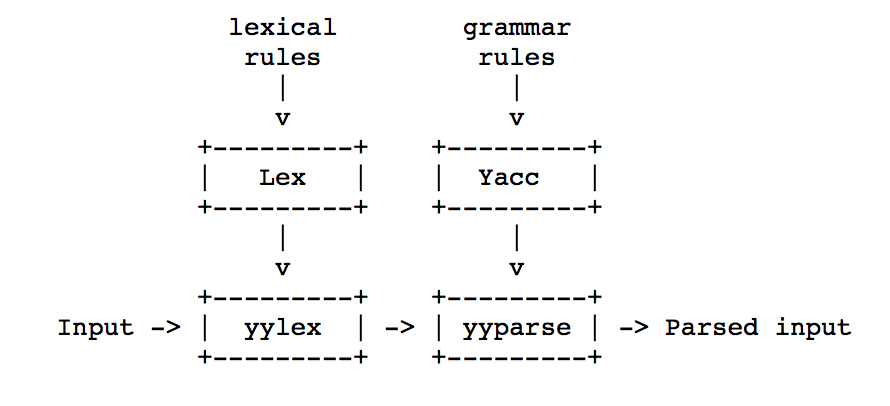
\includegraphics[scale=0.6]{images/schema_lex_yacc.png}
			\end{center}

		\subsubsection{Et dans notre projet ?}

			Lex et Yacc nous permettrons de vérifier la syntaxe du code ainsi que de colorer les mots clefs. \\
			Lorsque Yacc reconnaîtra des tokens envoyés par Lex, il exécutera la fonction dans laquelle la docstring permettant la 			reconnaissance des tokens est située.
			
			\begin{figure}[!h]
			
				\begin{center}
					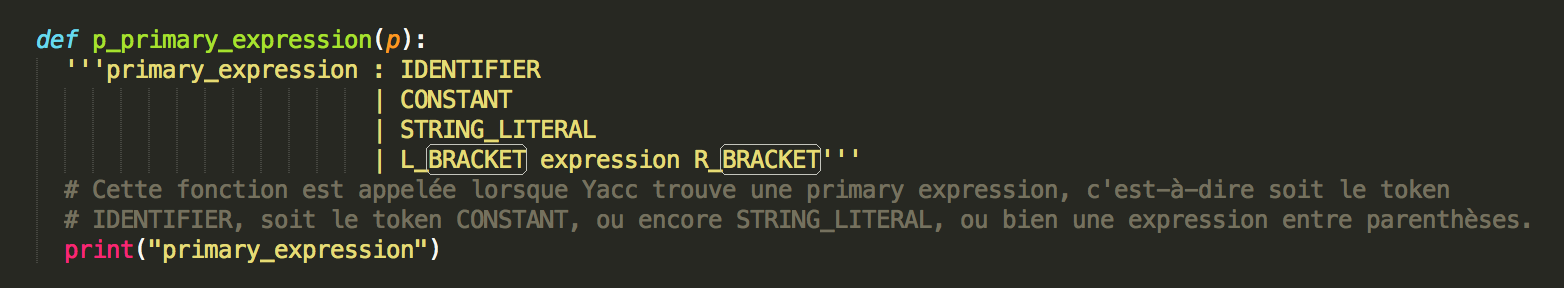
\includegraphics[scale=0.6]{images/exemple_fct_yacc.png}
					\caption{Exemple de fonction de reconnaissance YACC}
				\end{center}
			
			\end{figure}

\section{Séance 3, 07/10/16}

	Nous devons maintenant nous pencher sur l'analyse des sorties générées par Lex et Yacc. On doit les interpréter et les comprendre pour pouvoir les exploiter pour notre IDE. Nous devons également obtenir un arbre syntaxique abstrait grâce à l'analyse syntaxique afin de gérer l'auto-complétion.


	\subsection{Sortie de Lex}

		Lex génère donc une liste de token qui correspondent au type de chaque élément qu'il a reconnu grâce aux règles lexicales. Cette liste de token va nous permettre de colorer les mots en fonction de leur étiquettage. Pour notre IDE, nous allons donc utiliser Lex pour la coloration syntaxique. 
	
	\subsection{Sortie de Yacc}

		Yacc, en revanche, grâce à la liste de token récupérée par Lex, exécute la fonction dans laquelle est contenue la règle grammaticale si cette dernière est reconnue. Yacc va donc exécuter une action donnée lorsque la syntaxe du bloc d'instructions est correcte. Avec Yacc, nous allons par exemple pouvoir empêcher l'enregistrement du document en cours, si sa syntaxe n'est pas correcte.
		Pour l'instant, nous savons reconnaître les éléments seulement quand Yacc leur détecte une bonne syntaxe, mais c'est plus compliquée pour indentifier les éléments ayant une mauvaise syntaxe. C'est pour cela, que nous travaillons actuellement sur la sortie générée par Yacc. 
		
	\subsection{Analyse syntaxique produisant l'arbre syntaxique abstrait pour l'auto-complétion}

		Pour avoir l'arbre syntaxique abstrait permettant l'auto-complétion, nous devons utiliser YACC de PLY. Pour ce faire, nous avons mené des investigations et nous avons notamment trouvé des informations intéressantes sur ce site internet : \\\url{http://www.matthieuamiguet.ch/media/documents/MA-compil-03-Analyse_Syntaxique.pdf}. Nous sommes donc en train de voir actuellement comment implémenter cette analyse syntaxique à notre IDE afin d'obtenir l'arbre syntaxique abstrait pour gérer l'auto-complétion.
			
			\begin{figure}[!h]
			
				\begin{center}
					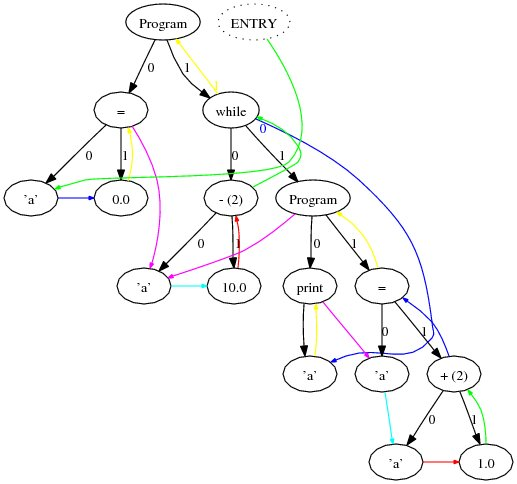
\includegraphics[scale=0.6]{images/AST.jpg}
					\caption{Exemple d'arbre syntaxique}
				\end{center}
			
			\end{figure}
			
		
	\subsection{Coloration syntaxique avec Lex}

		Afin de colorer le texte présent dans notre zone de saisie, nous avons utilisés Lex. Pour cela, nous parcourons la liste des tokens trouvés par Lex. Puis pour chaque token nous ajoutons une balise HTML (span) avec un attribut style permettant de changer la couleur du texte. La couleur dépend du type du token (Identifier, Keyword, Comment). 

		\newpage
			
			\begin{figure}[!h]
			
				\begin{center}
					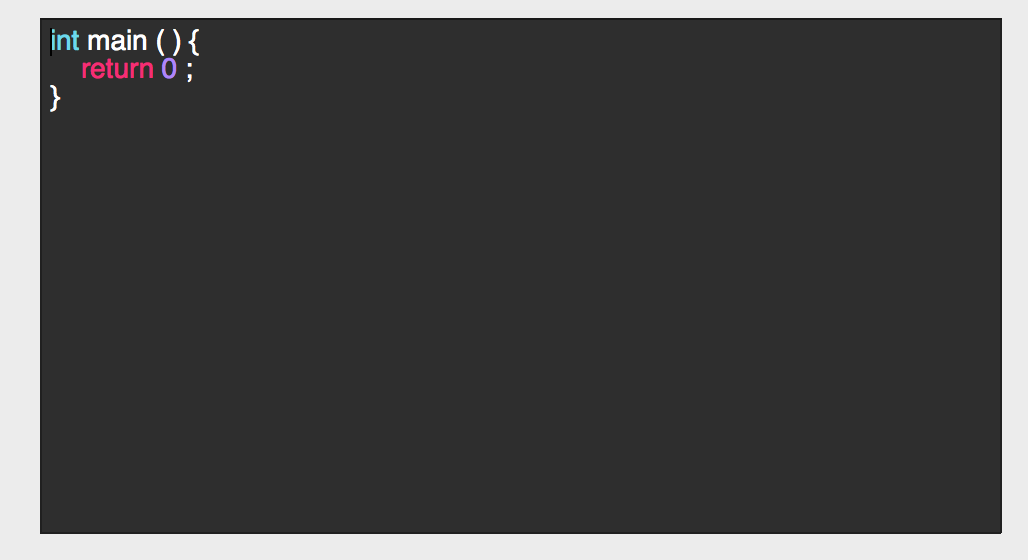
\includegraphics[scale=0.6]{images/coloration}
					\caption{Exemple de coloration syntaxique}
				\end{center}
			
			\end{figure}


			
					
			
\end{document}